\chapter{Locations}
\label{locations}
% 20 pages
Human mobility has been attracting a high degree of attention from numerous
study fields among which we find urban and traffic planning, traffic prediction,
the spreading of diseases and many others \cite{AsgariGB13} \cite{Brockmann08}.

The studies that have been conducted on this subject have been using various
ways to identify the travel behaviour of people. Some of them have focused on
studying the information gathered from observing the way in which money is
dispersed through time \cite{Brockmann06}, or they have been focusing in
studying the behaviour of mobile phone users by analyzing the way they move
based on the communication towers their phones are connecting to when they are
engaging in voice communication \cite{Barabasi08}. There are studies that try to
understand human mobility through the glass of social networks
\cite{yang2010using}, as it can be observed that individuals prefer to meet with
other people that are part of their community more often
\cite{Musolesi:2007:DMM:1317425.1317433}. GPS data has also been considered for
various studies \cite{cuttone2014inferring}, \cite{5657695}. The list of
elements that have been taken into consideration for trying to understand and
predict the way in which we are conducting our daily travels is far from being
short. 

\section{Wifi based positioning}

Even from the beginning of the 21st century, research has been actively
conducted for trying to use the Wifi system in order to determine real
positioning and different databases for positioning systems have been created.
These databases usually included the positions of the Wifi access points or RF
(radio-frequency) identified fingerprints \cite{Chen:2006:PMP:2166283.2166297}
\cite{Cheng:2005:ACM:1067170.1067195} \cite{Youssef:2005:HWL:1067170.1067193}
\cite{bahl2000radar}. Modern databases for Wifi positioning are created with
information about the signal strength for the Wifi access points and can
even have information about where they were discovered.

Koo et. al. \cite{koo2011autonomous} have explored an algorithm that can help
estimate the relative positions of access points corresponding to the real
geographic configuration with the help of multidimensional scaling techniques.
Considering the fact that access points are not able to tell real distances
between themselves and other access points, the study aims to estimate the
dissimilarities between different access points using scans. They have also
conducted an experiment in an office building in order to test the proposed
algorithm and the results showed an estimation error of approximately $7$ m.

Another study conducted in this similar direction is the one by Mok et. al.
\cite{mok2007location}. The authors explore the possibility of determining the
location of a device which can scan Wifi access points based on the signal
strength that the access points are displaying at the moment of the scan. They
estimate the positioning by performing a trilateration based on the information
the device gets from multiple access points. The accuracy for their algorithm
for the conditions that were present in their experiment was of about $1-3$ m.

Athanasiou et. al. \cite{athanasiou2009utilizing} give a very clear and
concrete description for two classes of wireless positioning systems. Their work
focuses on experimenting with parameters for these algorithms in order to find
the optimal solution in terms of accuracy under realistic settings. They also
adapt a global map matching algorithm in order to extract travel time maps from
wireless data and they propose a demonstration for showing that for high
sampling frequencies, the locations identified are comparable to the ones
derived from GPS data.

The two classes of algorithms that are explored by the authors are: centroid and
fingerprinting. \textit{Centroid} is presented as the fastest method for
positioning, however it depends on having the real location of the access
points. This information is in general unavailable and as such a proposed
solution is to estimate the locations of the access points by calculating an
arithmetic mean of all the coordinates at which it was visible. The
\textit{fingerprinting} method is based on the assumption that the access points
are stable over time (they do not change positions). This leads to the fact that
at any time, a measurement at a particular location will return the same list of
access points with the same signal strengths. As such, this list can be
considered as the unique fingerprint of the location.

% TODO add 2 figures for centroid and fingerprinting
Zhang et.al. \cite{zhang2012polaris} propose an algorithm based on
fingerprinting for estimating locations that takes into consideration the fact
that the signal strength from various access points does not necessarily stay
constant throught the time. They propose a way in which a similarity between
fingerprints can be calculated in order to determine if two fingerprints are in
fact representing the same location.

These are just a selection of works that have been conducted on finding a
solution for Wifi based positioning systems. With the growth and improvement of
Wifi systems, in time all barriers can be overcome and we could have a
positioning system that is as accurate yet considerably cheaper than GPS
positioning systems.

\section{Determining the fingerprint of a location}
In order to have a better understanding about the way in which the mobile phone
users have been moving throughout the experiment, we needed to have an image of
the way a given period of time would look based on their Wifi records from
SensibleDTU. As it has been presented in Section~\ref{data_structures}, the Wifi
data we are using for the present project consists in the following fields:
user id, timestamp, SSID, BSSID, RSSI and the context. However, considering the
amount of data involved, just by looking through the log files it is almost
impossible for us to understand at what moment the user might have reached a
location and when did they leave from it. In order to be able to do this, we
have created various visualizations considering different options, different
time frames and for multiple users in order to begin to understand what the data
can tell us, what can we use, what would we need and what can we discard when
moving further to defining what makes a location.

\subsection{Signal strength over time}

The first thing that we have tried to visualize was the access points (APs) that
were scanned by users' mobile phones throughout different periods of time. We
have plotted the APs and their registered signal strength for varied users in
order to see if we notice any patterns in their movements.

%userX == user 6
In Fig.~\ref{user_6_1d_lines} we can see how a day from the life of a random
user (referred to as userX) looks like. The day for which we have plotted the
data started on a Tuesday at $12:15$ pm and ends the next day right before the
same hour. The hourly intervals can be seen on the x axis, while the signal
strength values can be seen on the y axis. The legend contains the top $10$ most
popular~\footnote{An AP is more popular than another in case it appears more
times during the period of time for which the Wifi scans are analyzed}

\begin{figure}[h]
\centering
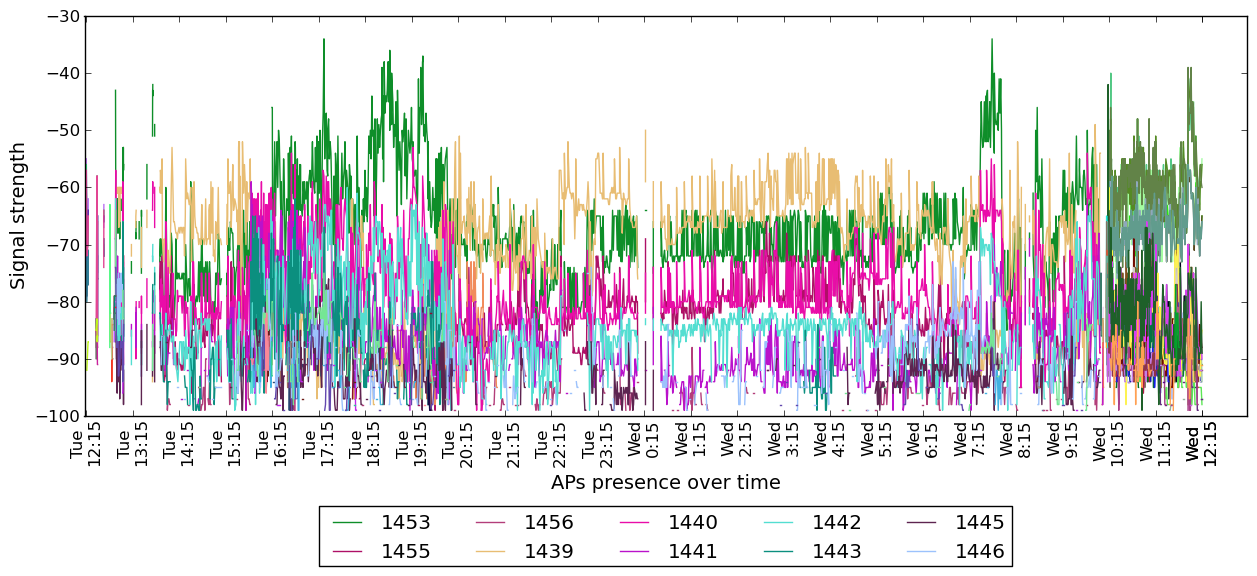
\includegraphics[height =
0.45\textwidth]{figures/user_6_sorted_1days_plot.png}
\caption{Example of the APs registered for an user throughout one day (using
connecting lines markers)}
\label{user_6_1d_lines}
\end{figure}

The steps for creating this type of visualization are as follows:
\begin{itemize}
  \item Retrieve data for the time duration for which the visualization is made
  \item Keep track of all the timestamps at which each AP has been seen and the
  AP's signal strength at that moment
  \item In case an AP is scanned no more than $2$ minutes after a it was
  previously scanned, then a line can unite the two moments in order to mark
  their proximity. If the apparitions are more than $2$ minutes apart there is
  a high possibility that there has been a location change or that the AP is
  experiencing technical problems and as such has stopped being active.
\end{itemize}

Although we have tried to visualize this type of information in various ways
(using different types of markers), we found that this way is the easiest to
interpret by people. If we leave out the lines, for example, as it can be seen
in Fig.~\ref{user_6_1d_point}, it is quite hard to interpret where location
might start or stop.

\begin{figure}[h]
\centering
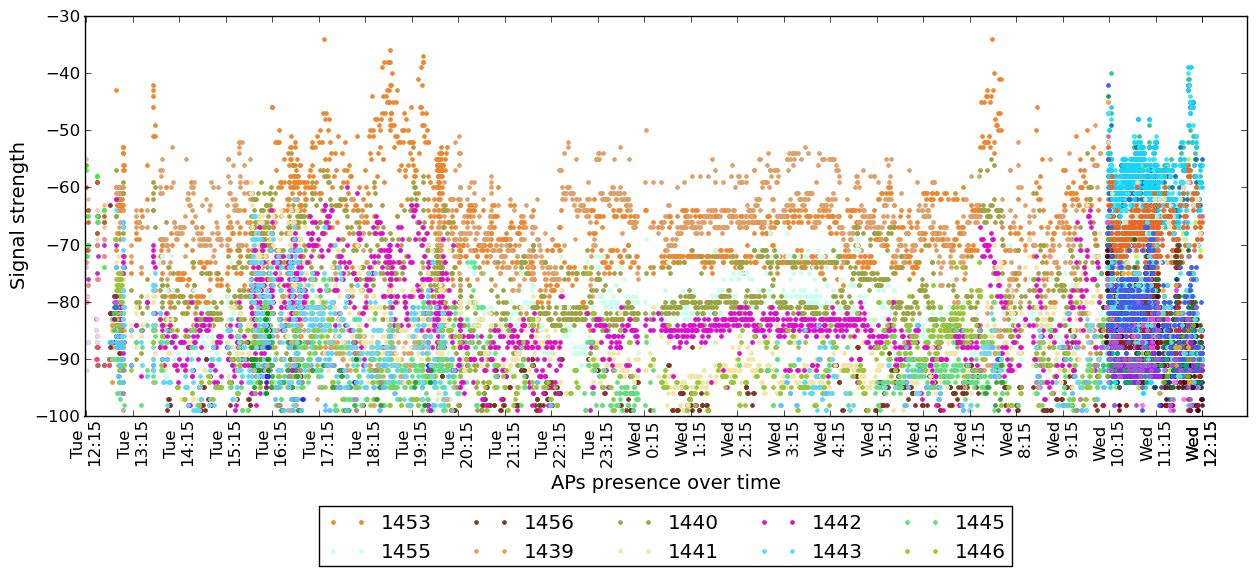
\includegraphics[height =
0.45\textwidth]{figures/point_user_6_sorted_1days_plot.png}
\caption{Example of the APs registered for userX throughout one day (using
point markers)}
\label{user_6_1d_point}
\end{figure}

Other ways in which we have been experimenting with visualization for this can
be found in Appendix~\ref{appendix_signal_strength}.

By looking at Fig.~\ref{user_6_1d_lines} we are at some level able to
distinguish moments of time at which the user seems to be arriving at a
location~\footnote{For example, we can say that what we notice from Wednesday
at 10:15 until the same day at 12:15 is different than anything we can see
before that time so we can assume that it is a new location.}, however is is
hard to nice any patterns because we are only observing a single day in the life
of userX. 

% user Y = user 3
Let us look at the data gathered through $7$ days from another user's (referred
to as userY) life. The visualization for this data can be seen in
Fig.~\ref{user_3_7d}. The image gives out some very interesting information. We
can, for example, notice the repeating patterns which are dominated by the
orange, light green and blue colors. These patterns appear during the evening
and the night and we can assume that the user is spending this time at the
location which we can label ``home''.

We can notice some periods of time that are free. These free gaps like, for
example, from Monday morning until Monday evening are gaps in which no signal
was scanned and can mean that either the mobile phone was closed or that the
user decided to switch off the Wifi.

\begin{figure}[h]
\centering
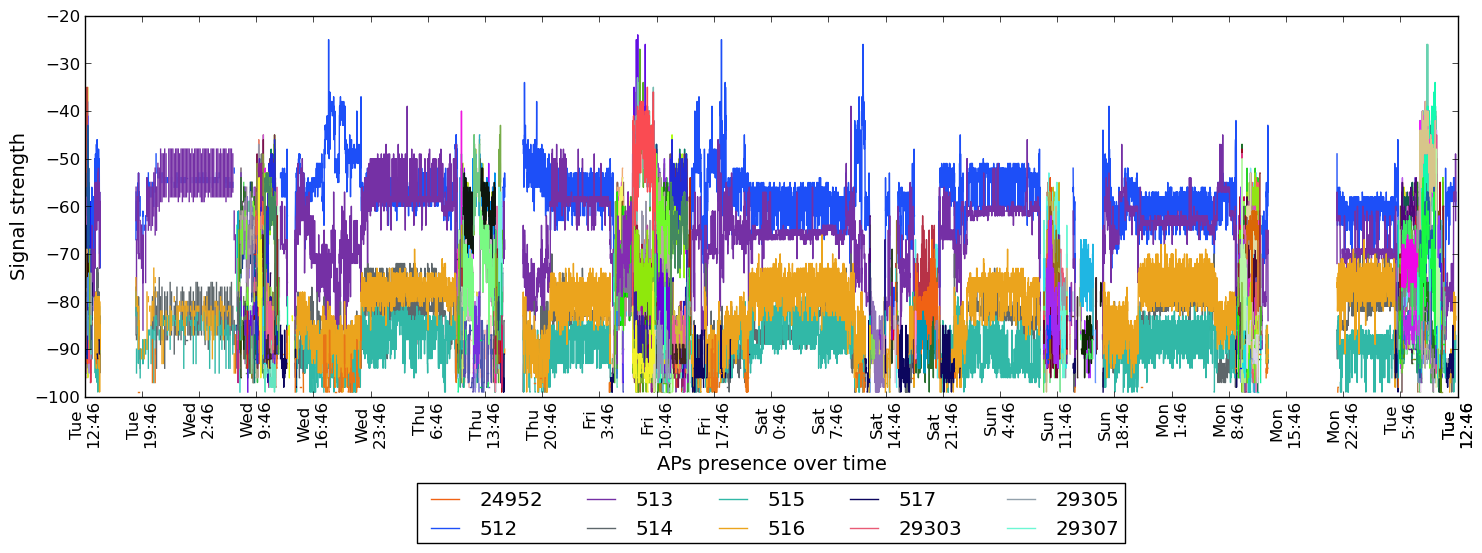
\includegraphics[height =
0.45\textwidth]{figures/user_3_sorted_7days_plot.png}
\caption{Example of the APs registered for userY throughout 7 days}
\label{user_3_7d}
\end{figure}

We can also notice fragments in which the density of signals is quite high, for
example on Wednesday morning. This means that the user was located in a place
which has a large number of APs near and since we can notice a regularity in
this pattern we can assume that this place can be the University. This might
seem unlikely based on the fact that the patterns sometimes is identified during
the night, however this particular week is set in October when there are
deadlines for school projects that need to be handed in.

As we can see, these visualization can offer us a good first glance at what the
locations might be like, yet they also make us consider other things that we can
learn about the data. For example:
\begin{itemize}
  \item How many samples from each access point are received during a given time
  frame
  \item What is the average signal for various time frames for a given access
  point
  \item What are the running averages for signals from various access point
\end{itemize}
%As we can see, these visualization can offer us a good first glance at what the
%locations might be like, however, they also raise some interesting questions.
%For example:
%\begin{itemize}
%  \item Can the spikes in the signals cause any problems in determining
%  locations?
%  \item Does the sample density give us additional useful information for
%  extracting the locations?
%\end{itemize}

\subsection{Sample density}

When trying to identify locations based on the Wifi data, it is important to
only take into consideration the access points that actively contribute to the
fingerprint of the mentioned location. Before cleaning our data (as it has been
described in Section~\ref{data_cleaning}), isolated observable access points can
appear and unnecessarily burden the algorithm used for extracting the locations.
The best way to identify such access points is by analyzing the sample
density~\footnote{We define the sample density for an access point as the number
of times it appears in scans over a predefined time bin.} of the samples that
are identified during scanning.

In order to determine the sample density for each AP, we need to define a time
bin over which the sample density needs to be calculated. We have calculated the
density considering a time bin of $5$ minutes as we can assume that this amount
of time can be considered the minimum duration for which a user needs to be
situated in approximately the same place in order for us to not consider that
the location is a transition instead of a stop location.% TODO verify
% supposition

%TODO - userZ is 6 - 1 day , day 1
In Fig.~\ref{rssi_6_2nd_day} we have the different APs and their RSSI values at
the different moments when the mobile phone has identified them in the scans for
an user referred to as userZ. In Fig.~\ref{samples_6_2nd_day} we can observe the
sample density for one of the APs that are predominant during the visualized
time frame. As we can see, the number of times the AP is present in the scans
throughout the day is quite high and it is registered during numerous different
periods during the day. We can easily assume that this AP is one of the key APs
that define one of the locations the user has been associated with.

\begin{figure}[h]
\centering
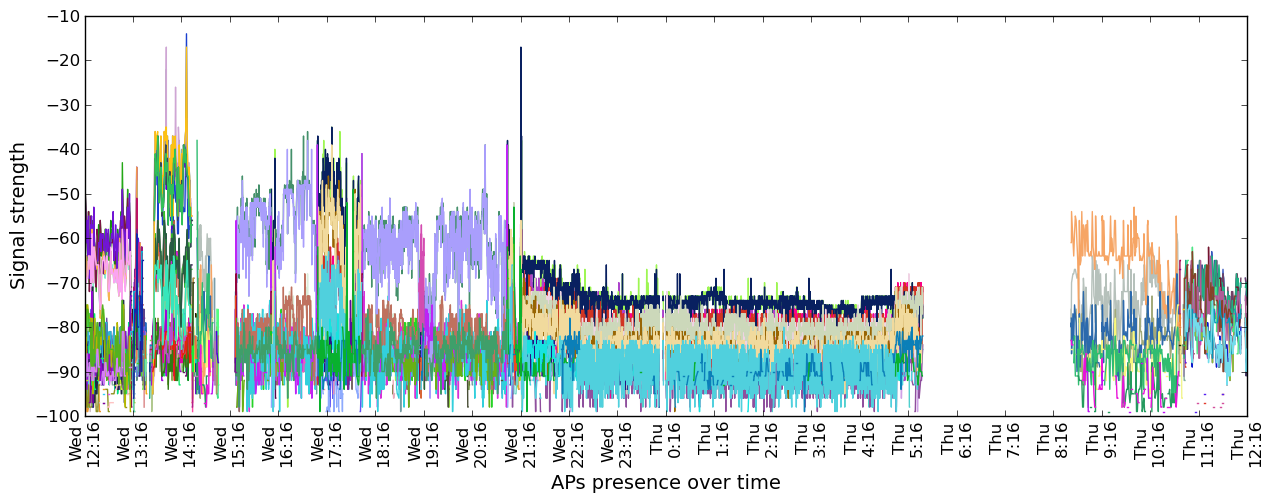
\includegraphics[width =\textwidth]{figures/combinations/user_6_sorted_1days_plot_croped.png}
\caption{Example of the APs registered for userZ throughout 1 day}
\label{rssi_6_2nd_day}
\end{figure}

\begin{figure}[h]
\centering
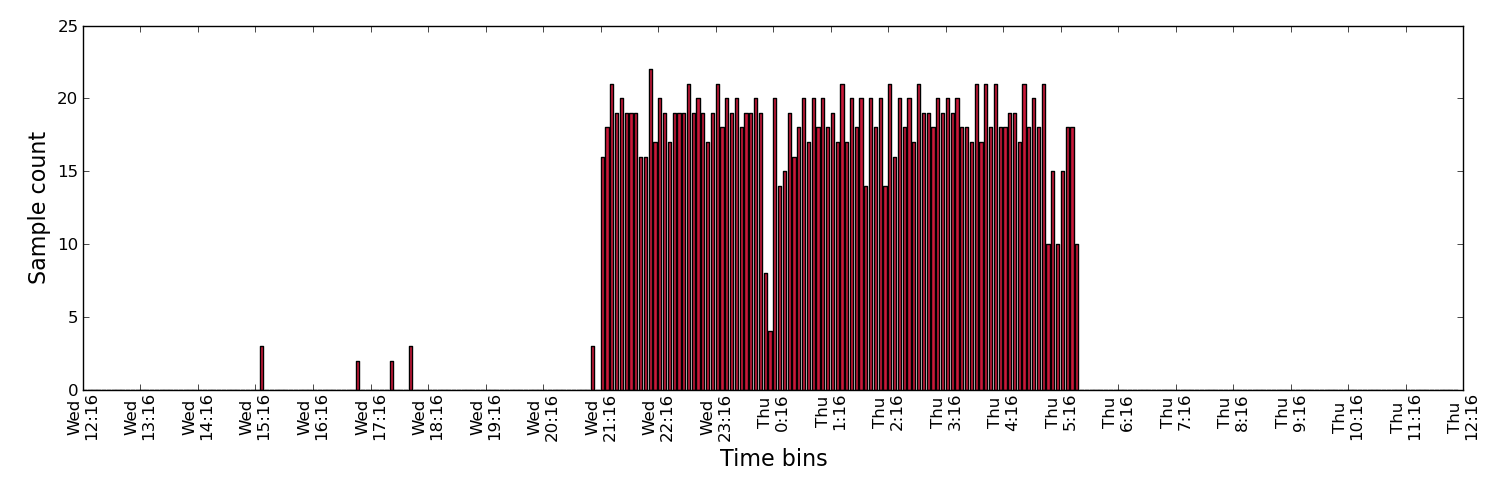
\includegraphics[width =\textwidth]{figures/combinations/user_6_sorted_1days_plot_14280_histo.png}
\caption{Example of an AP which appears often}
\label{samples_6_2nd_day}
\end{figure}

On the opposite end as number of times it has appeared during the scans, we have
the AP in Fig.~\ref{few_samples_6_2nd_day}. As it can be seen, this AP only
appears $5$ times over a one single $5$ minute time bin. We can easily presume
that the presence or absence of this particular AP will not offer us relevant
information over the location at which the user was situated when it appeared in
the scans. This statement is also sustained by the fact that the user location
seems to be consisted from Wednesday $12:16$ up until around $13:16$ according
to what we can observe in Fig.~\ref{rssi_6_2nd_day}, even though the AP does not appear
throughout most of this time.

\begin{figure}[h]
\centering
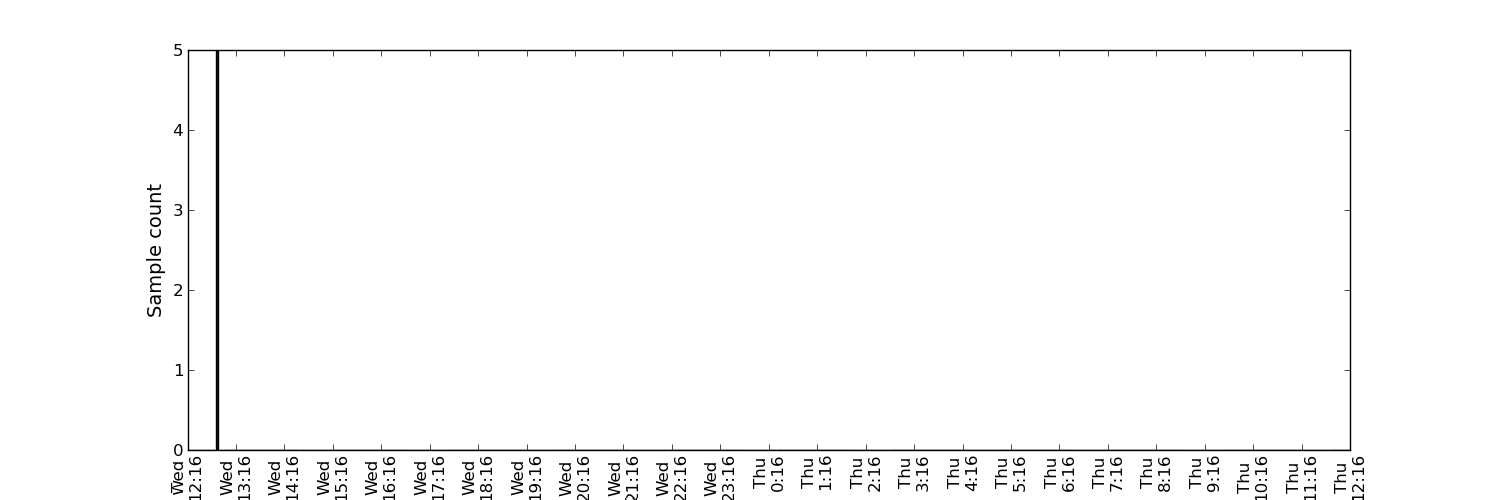
\includegraphics[width =\textwidth]{figures/combinations/1553_modif.png}
\caption{Example of an AP that appears just a few times}
\label{few_samples_6_2nd_day}
\end{figure}

Other examples of visualizations for APs based on their sample density can be
found in Appendix~\ref{appendix_sample_density}% TODO - add stuff to appendix
% TODO - modify and add fig with only one apparitions with 5 samples in 5
% minutes -> to modify and say we take into consideration only those with more
% than 5 samples in 5 minutes

\subsection{Exploring the implications of the signal strength}
Something that is often taken into consideration during studies regarding the
determination of locations based on Wifi data is the value which indicates
the signal strength received from the various APs. The level of the signal
strength indicator can, in general, give us a good approximation of how close we
are to a particular AP. However, Wifi networks are susceptible to interferences
\cite{MahantiCWA10}, meaning that there numerous factors which can cause signals
to spike even in case the device which scans the region for AP signals does not
move. This can represent a factor of risk when including the signal strength
value in the location extraction from Wifi data as the same location could be,
at different times, be associated to an AP which has a signal strength that
oscillates based on other external factors.

In order to see if we can smooth down possible fluctuations we have employed two
mathematical tools. We have calculated the average signal strength, as well as
the running average, considering different length time bins.

\subsection{Average signal strength}
\label{average_sig}

In order to calculate the average signal strength of a given AP for a given time
bin, we needed to identify all the moments of time inside the given time bin in which
the AP has been spotted during the scans. The average signal of the AP is
calculated as the sum of all the strength values that have been recorded for the
AP inside the time bin and the sum is then divided to the number of recorded
apparitions of the AP. For example, if we were to have an AP which appears 6
times inside a $5$ minutes time bin with the following RSSI values [-60, -70,
-60, -80, -90, -60], then the average signal strength for this particular time
bin for our AP would be $avg = [(-60) + (-70) + (-60) + (-80) + (-90) +
(-60)] / 6= -70$ dBm.

We have calculated the average signal for various users and various days. We
have also calculated it for different time bin length. For example, for the same
data that we can see in Fig.~\ref{rssi_6_2nd_day} and for the same AP that has
the sample density represented in Fig.~\ref{samples_6_2nd_day}, if we visualize
the non-null averages calculated for time bins of $5$ minutes, we would have the
representation in Fig.~\ref{user_6_avg_1d_5m}. The X axis records the time
while on the Y axis records the values of the averages

% TODO plot only with this AP in normal mode and maybe make some observations.
%TODO add more to appendix.

\begin{figure}[h]
\centering
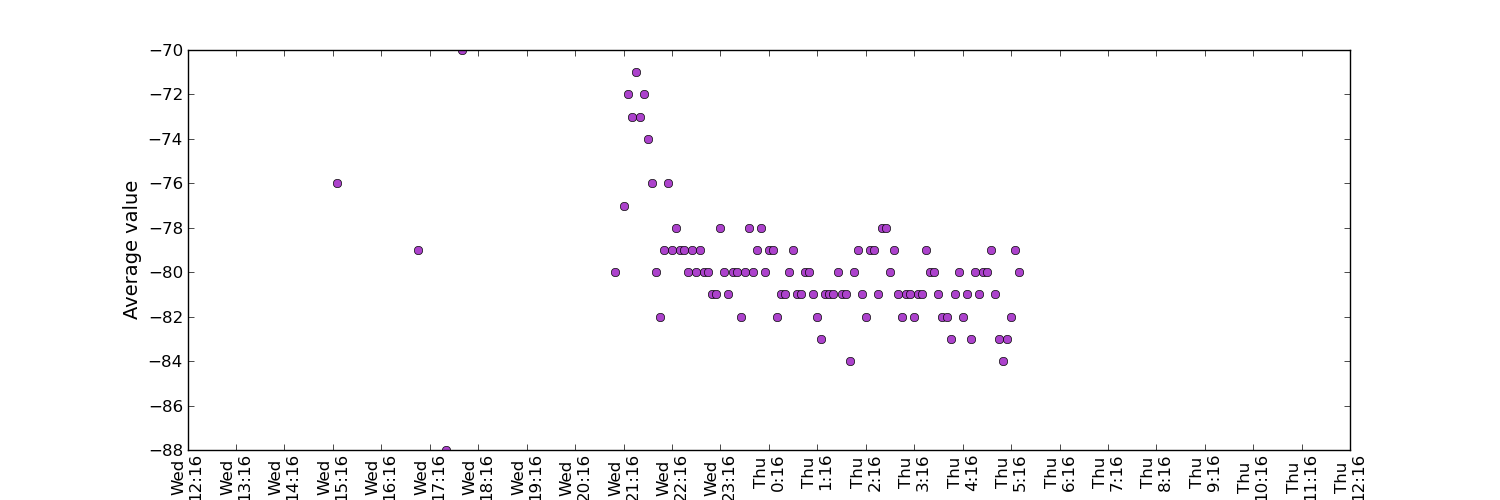
\includegraphics[width =\textwidth]{figures/combinations/user_6_sorted_1days_plot_14280_avg_sig.png}
\caption{Example of average signal strength visualization for userZ}
\label{user_6_avg_1d_5m}
\end{figure}

The averages are represented by big dots symbols which appear at the beninning
of the time bin for which the average is calculated. For example, if we have
calculated an average for the interval $12:05 - 12:10$, the average is plotted
on the visualization at $12:05$. 

Additional examples of averages for different APs scanned during the same day by
userZ's mobile phone can be found in Appendix~\ref{appendix_signal_strength}.

\subsection{Running average signal strength}
The average signal brings a small improvement as far as eliminating the signal
spikes go, however, an even better way in order to smooth out any signal
fluctuations is to calculate the running average\footnote{Also referred to as
the moving average} \cite{Hyndman09movingaverages}.

We have calculated the running average for different users and time frames, and
we have taken into consideration different time bins when calculating it.
The algorithm for calculating it is as follows:
\begin{itemize}
  \item For the selected user and the selected time frame, we have extracted for
  each AP the time stamps at which it has been identified by the user's phone
  \item We have divided for each AP the previously mentioned time stamps into
  bins of $2$, $5$ or $10$ minutes recording also the signal
  strength identified at each time stamp\footnote{By doing this we have the
  signal strength for the given AP at any moments it has appeared inside the time bin}
  \item The above identified time bins are overlapping. For example, if a
  sequence of signals $[-60, -80, -70, -70]$ that have each been identified at $1$ minute
  apart is to be divided into bins of $2$ minutes, the resulting $2$
  minute bins would be: $[-60, -80]$, $[-80, -70]$, $[-70, -70]$
  \item The running average is calculated as the sum of the values present in a
  time bin which is then divided to the number of values. For example, for the
  above time bins, the running averages would be $-70$, $-75$ and $-70$
\end{itemize}

In Fig.~\ref{user_1_APs_1d} we can see the APs associated with another user
(referred to as userT) and their signal strengths over a day.
Fig.~\ref{user_1_AP85_1d} shows the signal strength for just one of the
identified APs. The average signal as is presented in Section~\ref{average_sig}
for the same AP can be seen in Fig.~\ref{user_1_AP85_avg_1d}.
Fig.~\ref{user_1_AP85_rn2avg_1d}, Fig.~\ref{user_1_AP85_rn5avg_1d} and
Fig.~\ref{user_1_AP85_rn10avg_1d} present the running averages calculated for
the same AP for time bins of $2$, $5$ and $10$ minutes~\footnote{In this
representation, only the non-null values for running averages are displayed}.
The X axis of these figures track the succession of time moments while the Y
axis keeps track of the value of the running average calculated over this time.

\begin{figure}[!h]
\centering
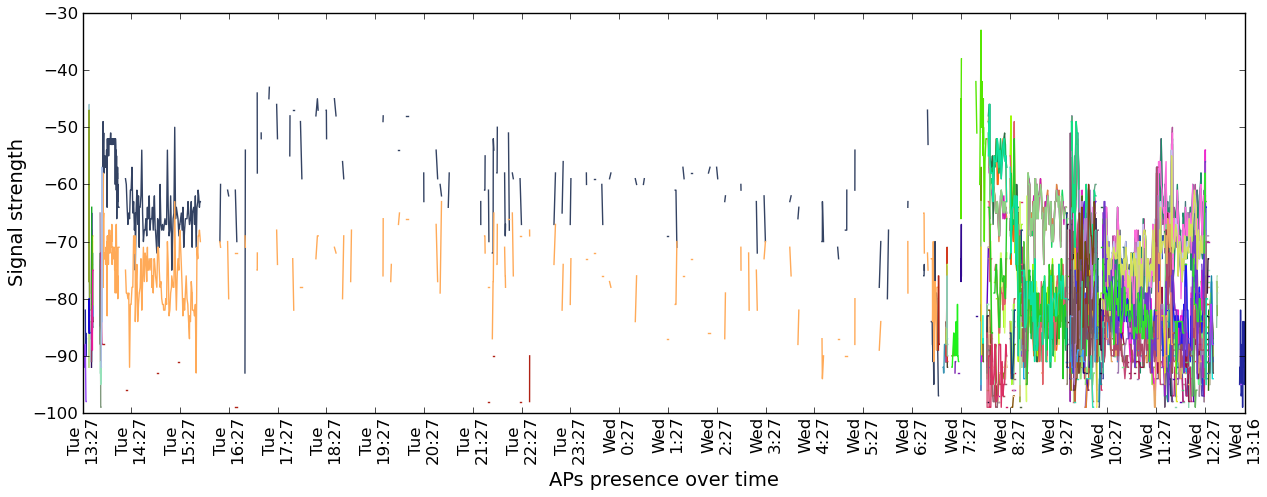
\includegraphics[width
=\textwidth]{figures/rn_avg/user_1_sorted_1days_plot.png}
\caption{Example of APs presence over time for userT}
\label{user_1_APs_1d}
\end{figure}

\begin{figure}[!h]
\centering
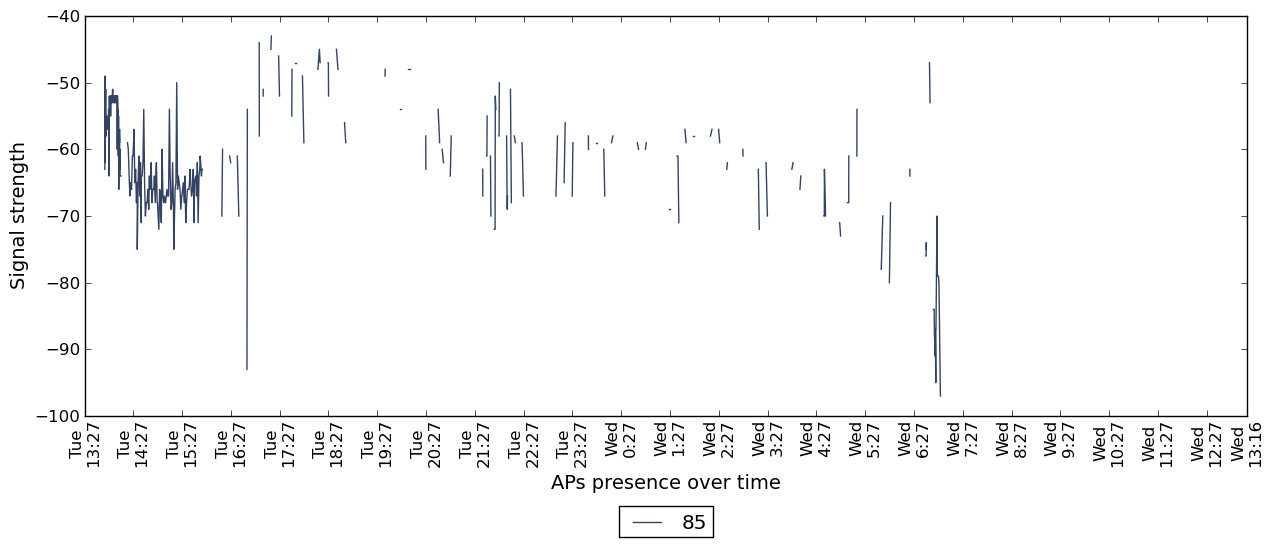
\includegraphics[width
=\textwidth]{figures/rn_avg/user_1_sorted_85_plot.png}
\caption{AP 85 for userT during 1 day}
\label{user_1_AP85_1d}
\end{figure}

\begin{figure}[!h]
\centering
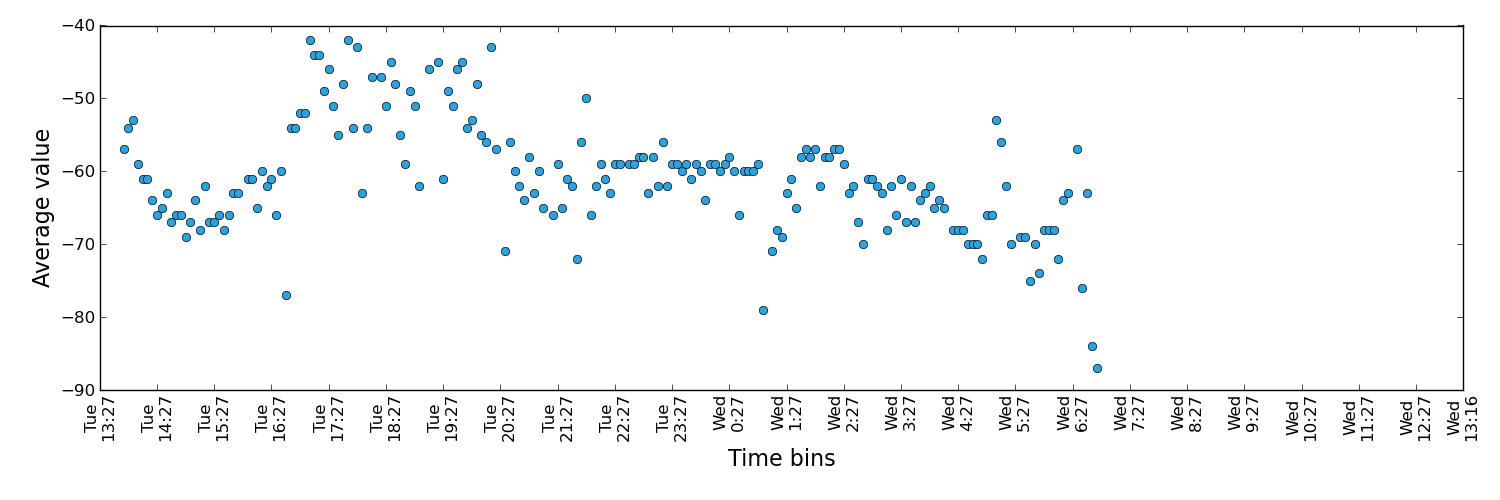
\includegraphics[width
=\textwidth]{figures/rn_avg/user_1_sorted_1days_plot_85_avg_sig.png}
\caption{Average strength for AP 85 for userT during 1 day}
\label{user_1_AP85_avg_1d}
\end{figure}

\begin{figure}[!h]
\centering
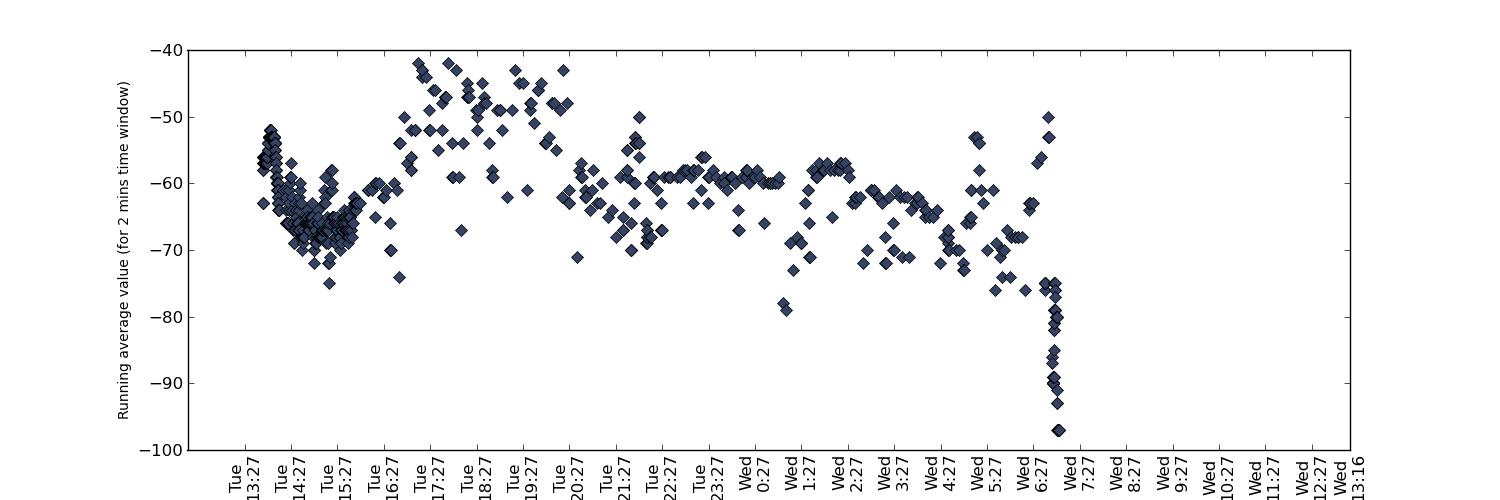
\includegraphics[width
=\textwidth]{figures/rn_avg/user_1_sorted_1days_plot_85_rn_avg_sig_2.png}
\caption{Running average for AP 85 for userT during 1 day (2 minute time bins)}
\label{user_1_AP85_rn2avg_1d}
\end{figure}

\begin{figure}[!h]
\centering
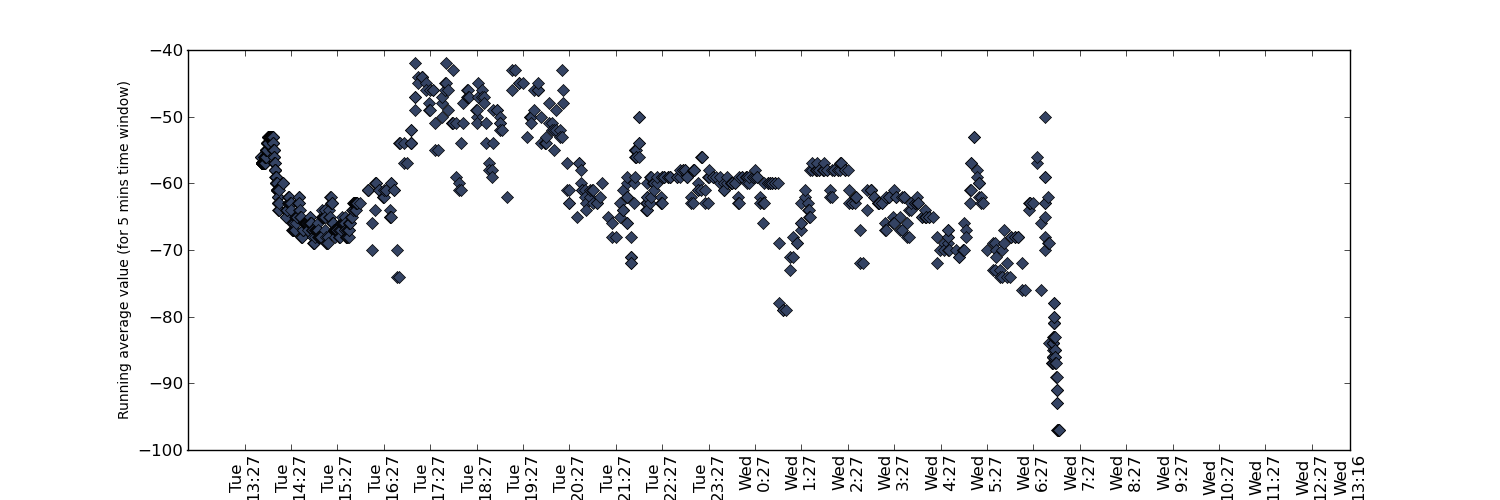
\includegraphics[width
=\textwidth]{figures/rn_avg/user_1_sorted_1days_plot_85_rn_avg_sig_5.png}
\caption{Running average for AP 85 for userT during 1 day (5 minute time bins)}
\label{user_1_AP85_rn5avg_1d}
\end{figure}

\begin{figure}[!h]
\centering
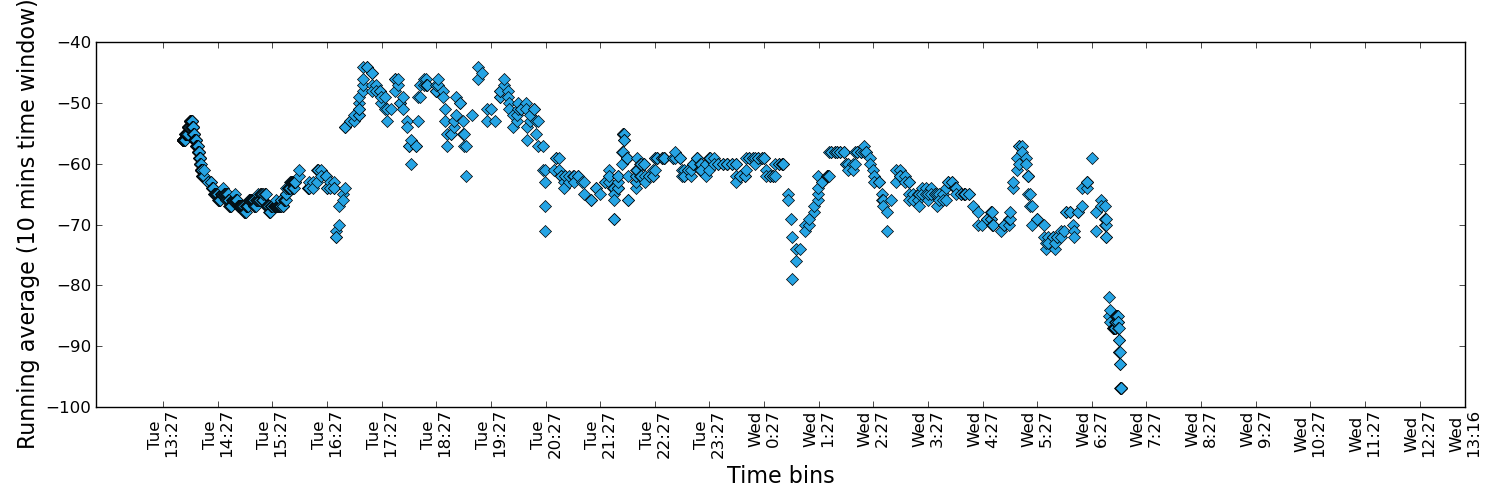
\includegraphics[width
=\textwidth]{figures/rn_avg/user_1_sorted_1days_plot_85_rn_avg_sig_10.png}
\caption{Running average for AP 85 for userT during 1 day (10 minute time bins)}
\label{user_1_AP85_rn10avg_1d}
\end{figure}

The way in which the fluctuations are smoothed down can be easily seen in the
figures that present the running averages calculated for various time bins. The
fluctuations are smoother as the time bin is increased.

Visualizations for running averages calculated for other APs identified during
the same day for userT can be found in Appendix~\ref{appendix_rn_avg}.

\subsection{Signal presence}
\label{sig_pres}

Even though averaging the signal strength through time improves at a certain
level the fluctuations in the signal strength, in a real environment spikes will
always be present and this will bring extra difficulties in estimating locations
based on fingerprints that contain the value of the signal strength for the
involved APs.

Another way of looking at locations is by calculating their fingerprint based
only on the identity of the APs that have been identified while the user was
found at that particular location. Basically, instead of defining a location
based on both the identity of the APs present and their signal strength, we
would only associate locations to visible APs.

The idea is simple and elegant and has been used in previous studies with
success \cite{Larsen:2009:MCT:1813042.1813063}. The concept behind is that, in
general\footnote{New APs can be set up or old ones can be changed with new ones
in time, which would mean a change in how the scans would look for the same
location. However, this is an issue that is outside the scope of the present
paper and work.}, at a given location the scans will always show the presence of
the same APs. If, after a time, the scans change and other APs appear, it is
reasonable to assume that the user has changed locations.

Since the information offered by the signal strength does not seem to be of the
ultimate importance, we can, in this case, try to identify the locations only
based on the presence of the APs. We consider that an AP is present at a
specific moment of time if the Wifi scans at that moment register a signal
strength from that AP. However, as it has been mentioned previously, due to
interferences, the signal from the AP might be lost for short periods of time
even when the user does not change their location.Considering this and the
assumption that, in general, people tend to spend at least a few minutes in a
stop location (otherwise meaning that they might be just transiting it), we have
made the decision to adapt for our case the definition for the presence of an
AP.

We divide our data into time bins of $5$ minutes~\footnote{We consider 5 minutes
as the minimum amount of time that needs to be spent in a location for it be
considered a stop location. This number can be easily adjusted in case further
research shows that it is not the optimal assumption.}. We redefine the presence
of an AP as follows: an AP is considered to be present for the duration of a $5$
minute time bin if it appeared in the scans at any point inside this time
interval.

We can use visualization in order to see how this transforms the way in which we
can understand the data. In Fig.~\ref{} we have the different APs that have been
scanned throughout the duration of $2$ days for userX. In Fig.~\ref{} we can see
the top $50$ predominant APs and their presence over $5$ minutes time bin during
the same $2$ days~\footnote{We restrict our visualization to $50$ APs as it
would be hard to understand an image in which we would be displaying all the
hundreds of APs which were encountered throughout the $2$ days.}. The X axis
keeps track of the time bins throughout the $2$ days, while the Y axis
represents the annonymized identifiers for the APs.

\begin{figure}[!h]
\centering
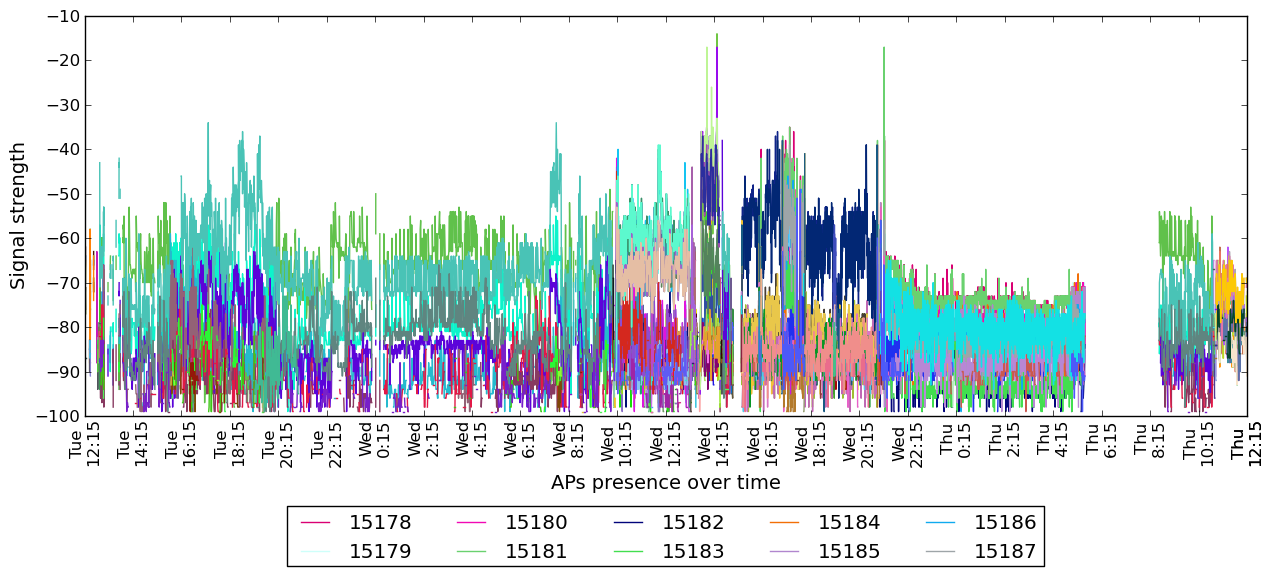
\includegraphics[width
=\textwidth]{figures/presence/user_6_sorted_2days_plot.png}
\caption{Scanned APs for userX throughout a duration of 2 days}
\label{user_6_APs_2d}
\end{figure}

\begin{figure}[!h]
\centering
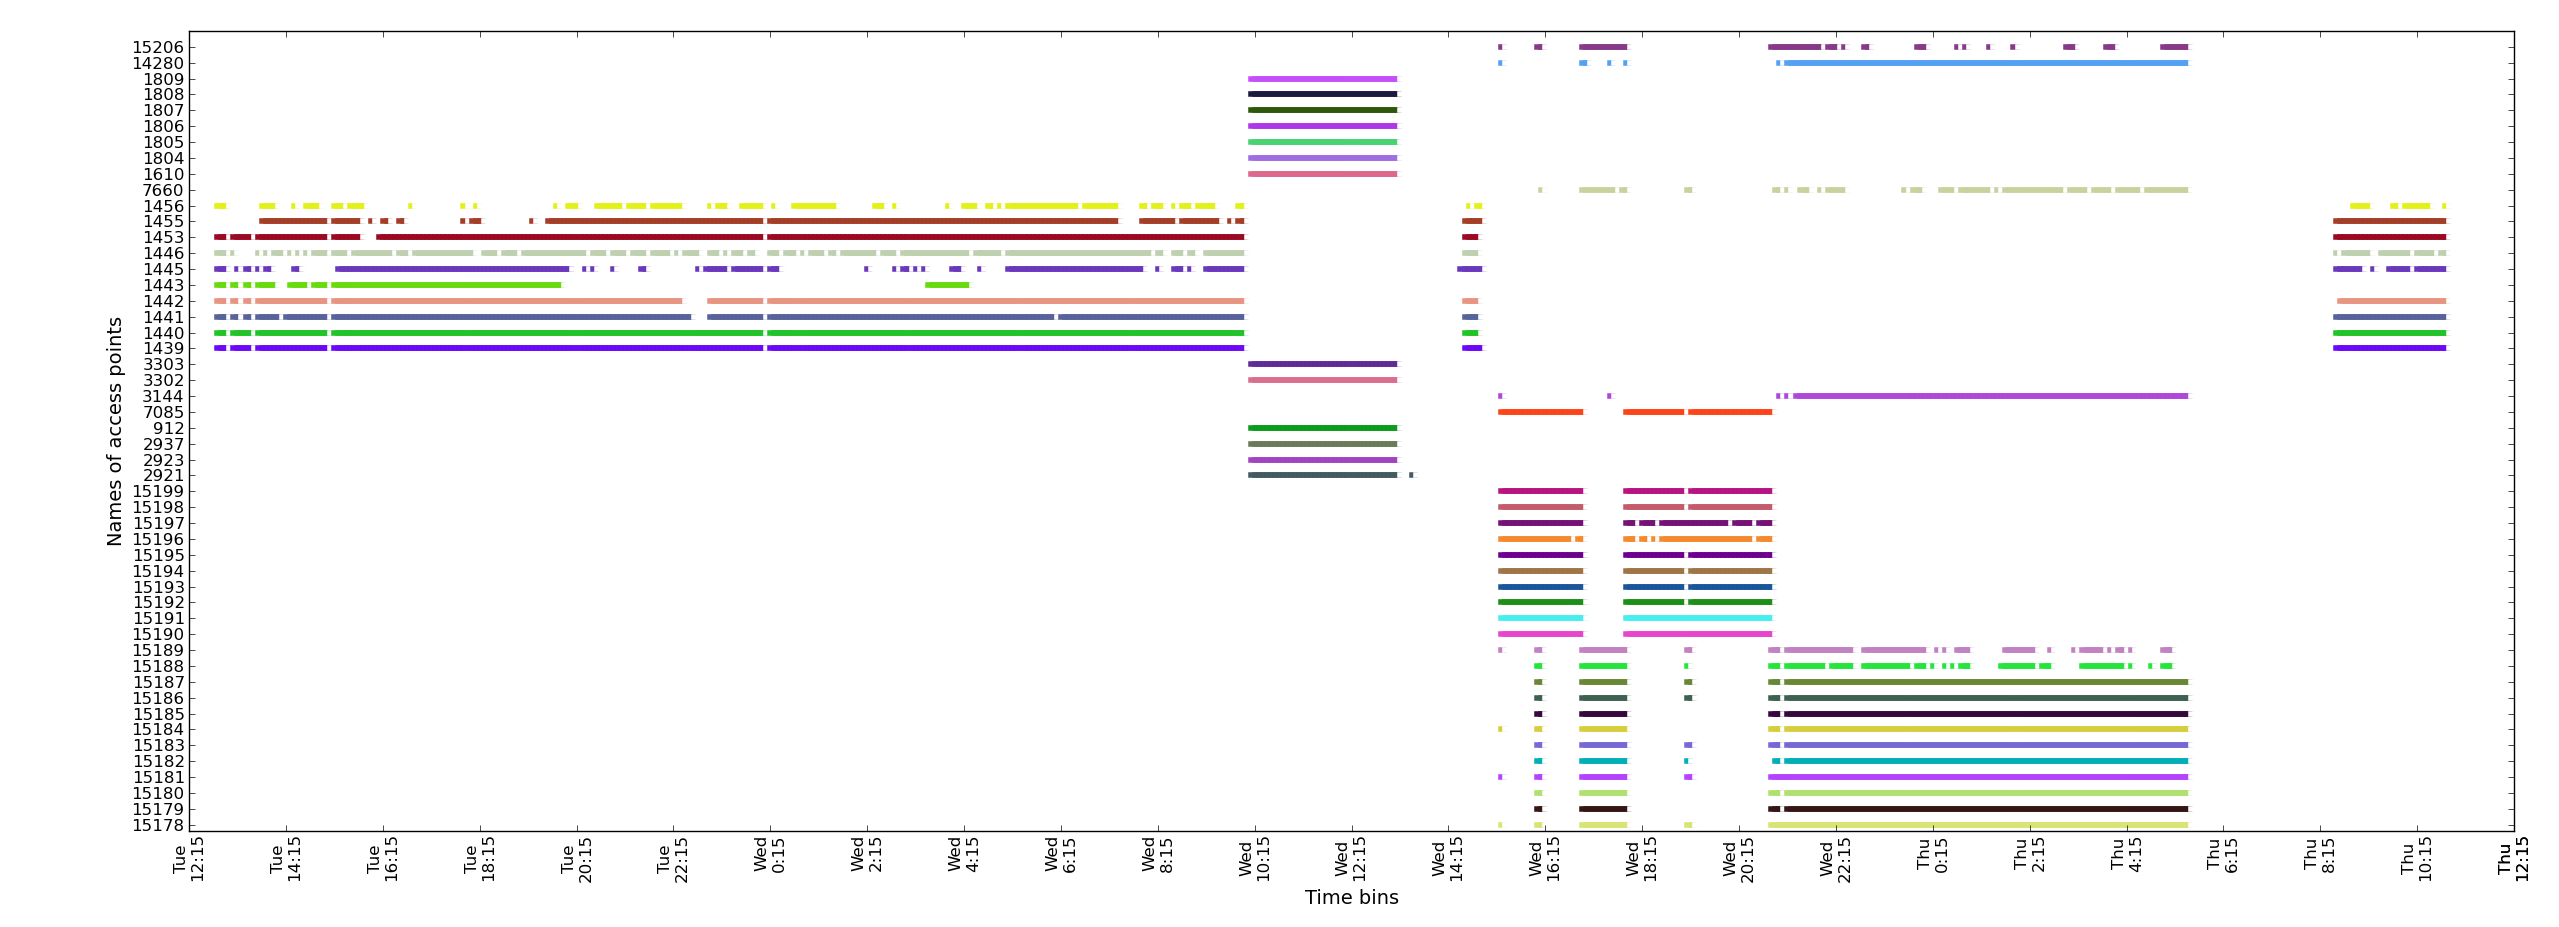
\includegraphics[width=1\textwidth]{figures/presence/user_6_sorted_2days_no_rssi_plot_crop.png}
\caption{The most common 50 APs for userX during the given 2 days (presence
visualization calculated for 5 minutes time bins)}
\label{user_6_pres_2d}
\end{figure}

By closely observing the two visualization, it is quite easy to see that indeed
they are representations of the same period of time. Even if not all APs are
displayed in the visualization for the presence of the APs over time, we can
notice that, for example, the user has spent the time from Wednesday $21:15$
until almost Thursday $6:15$ in one location. This also coincides with what we
can observe in the visualization for all the APs (with signal strength) scanned
throughout this time.

In Appendix~\ref{appendix_pres} can be found a visualization for the presence
of APs for a period of $2$ days for another user. The presence for APs is determined for $5$
minutes time bins over the $2$ days.

\section{Extracting locations}

By visualizing the Wifi data in the way presented in Section \ref{sig_pres}, we
can begin to see how locations seem to succeed each other throughout the days of
a particular user. However, it is important to be able to implement a solution
that will extract these locations from a large amount of data so that we would
not be needed to examine the data manually. We have used different methods in
order to get the best possible approximation for identifying the locations. The
methods we have tried are: using \textit{networks}, using \textit{k-means
clustering} and using \textit{Hidden Markov Models}.

\subsection{Network theory}

Networks have a high degree of importance when trying to understand human or
animal behaviour. They have been used in combination with social platforms in
order to extract a new definition of friendship \cite{cho2011friendship}, they
have been used for monitoring animal behaviour \cite{4116628}, or to understand
the economical situations cause by the way in which people interact
\cite{Copic05identifyingcommunity}, or just to understand underlying communities
of people. During our research, we have considered the use of network theory in
order to extract locations from Wifi data.

In theory, we can expect that the APs that are identified at a particular
location will not appear in the scans the user's phone will have from another
location. This assumption is sound as the APs will rarely be moved and as such
they should always be associated to the same place. In this case, we should
expect that the succession of locations can be similar to what we can see in
Fig.~\ref{user_6_tn}., where AP1-AP6 are associated to location number 1, while
the remaining APs are associated with location 2 and the APs never overlap.

\begin{figure}[!h]
\centering
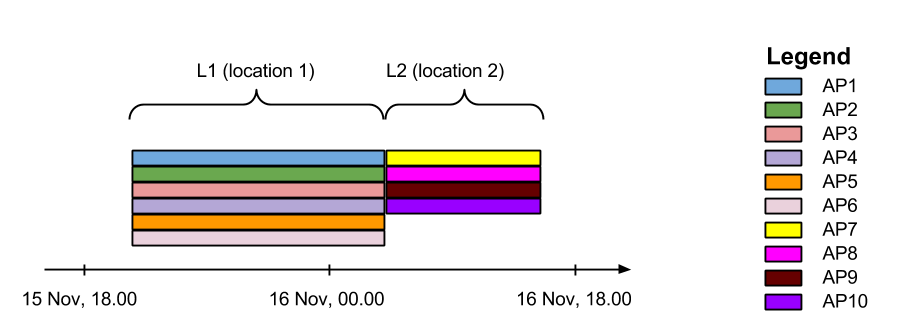
\includegraphics[width=1\textwidth]{figures/networks/theoretical_network.png}
\caption{Example of how, in theory, locations should be displayed through the
presence of APs}
\label{user_6_tn}
\end{figure}

The idea behind constructing the network  that can be used to extract the
locations is simple. A graph can be created for each user from their data and
the locations can be identified as follows:
\begin{itemize}
  \item We consider each found AP from the user data as a node in the created
  graph
  \item We construct a presence matrix for the identified APs. Each line in the
  presence matrix is associated to an AP and contains the signal presence
  (Section \ref{sig_pres}) calculated for the AP considering $5$ minute time bins
  throughout the time we are evaluating
  \item For each time bin, we identify the APs that are present trough it and
  we connect each two of them with an undirected edge (in case they have not
  been connected at a previous time)
  \item Since signal from various APs can be lost due to interferences, for each
  two APs for which we have created a connecting edge, we keep and update a
  variable which represents the number of times the APs have been identified in
  the same time bin
  \item After the network is completely created, we normalize the counts of how
  many times each two APs have been seen in the same time bin by dividing the
  counted value to the maximum number of apparitions of either of the two access points
  \item After the normalization we remove the weak links~\footnote{In this
  case, a link is considered weak if after normalization its associated value is
  below a given threshold}
  \item We consider the resulting connected components to be the extracted
  locations
\end{itemize}

An example on how to construct such a graph if given four APs and their
presence matrix can be seen in Fig.~\ref{network_calc_example}

\begin{figure}[!h]
\centering
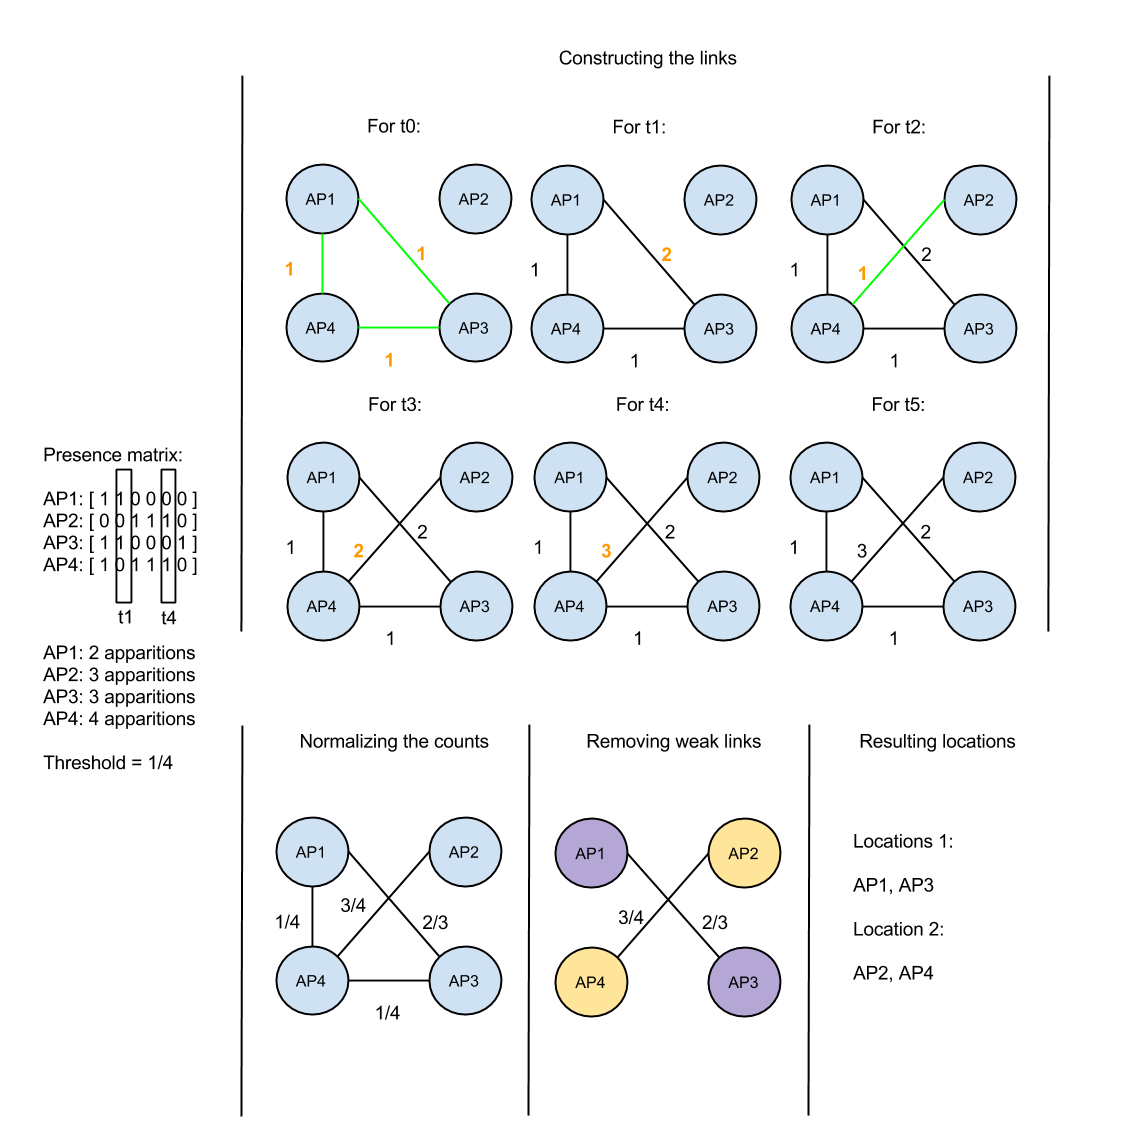
\includegraphics[width=1\textwidth]{figures/networks/net_constr_ex.png}
\caption{Example of constructing a network}
\label{network_calc_example}
\end{figure}

We have applied the previously described algorithm for a selection of users, but
the results have not been satisfactory.

For example, we can take data for one day for userX. The visualization for the
identified APs and their presence throughout this time can be observed in
Fig.~\ref{user_6_pres_1d}. By looking at this image, we can observe that the
user has been in $2$ main locations during this day.

\begin{figure}[!h]
\centering
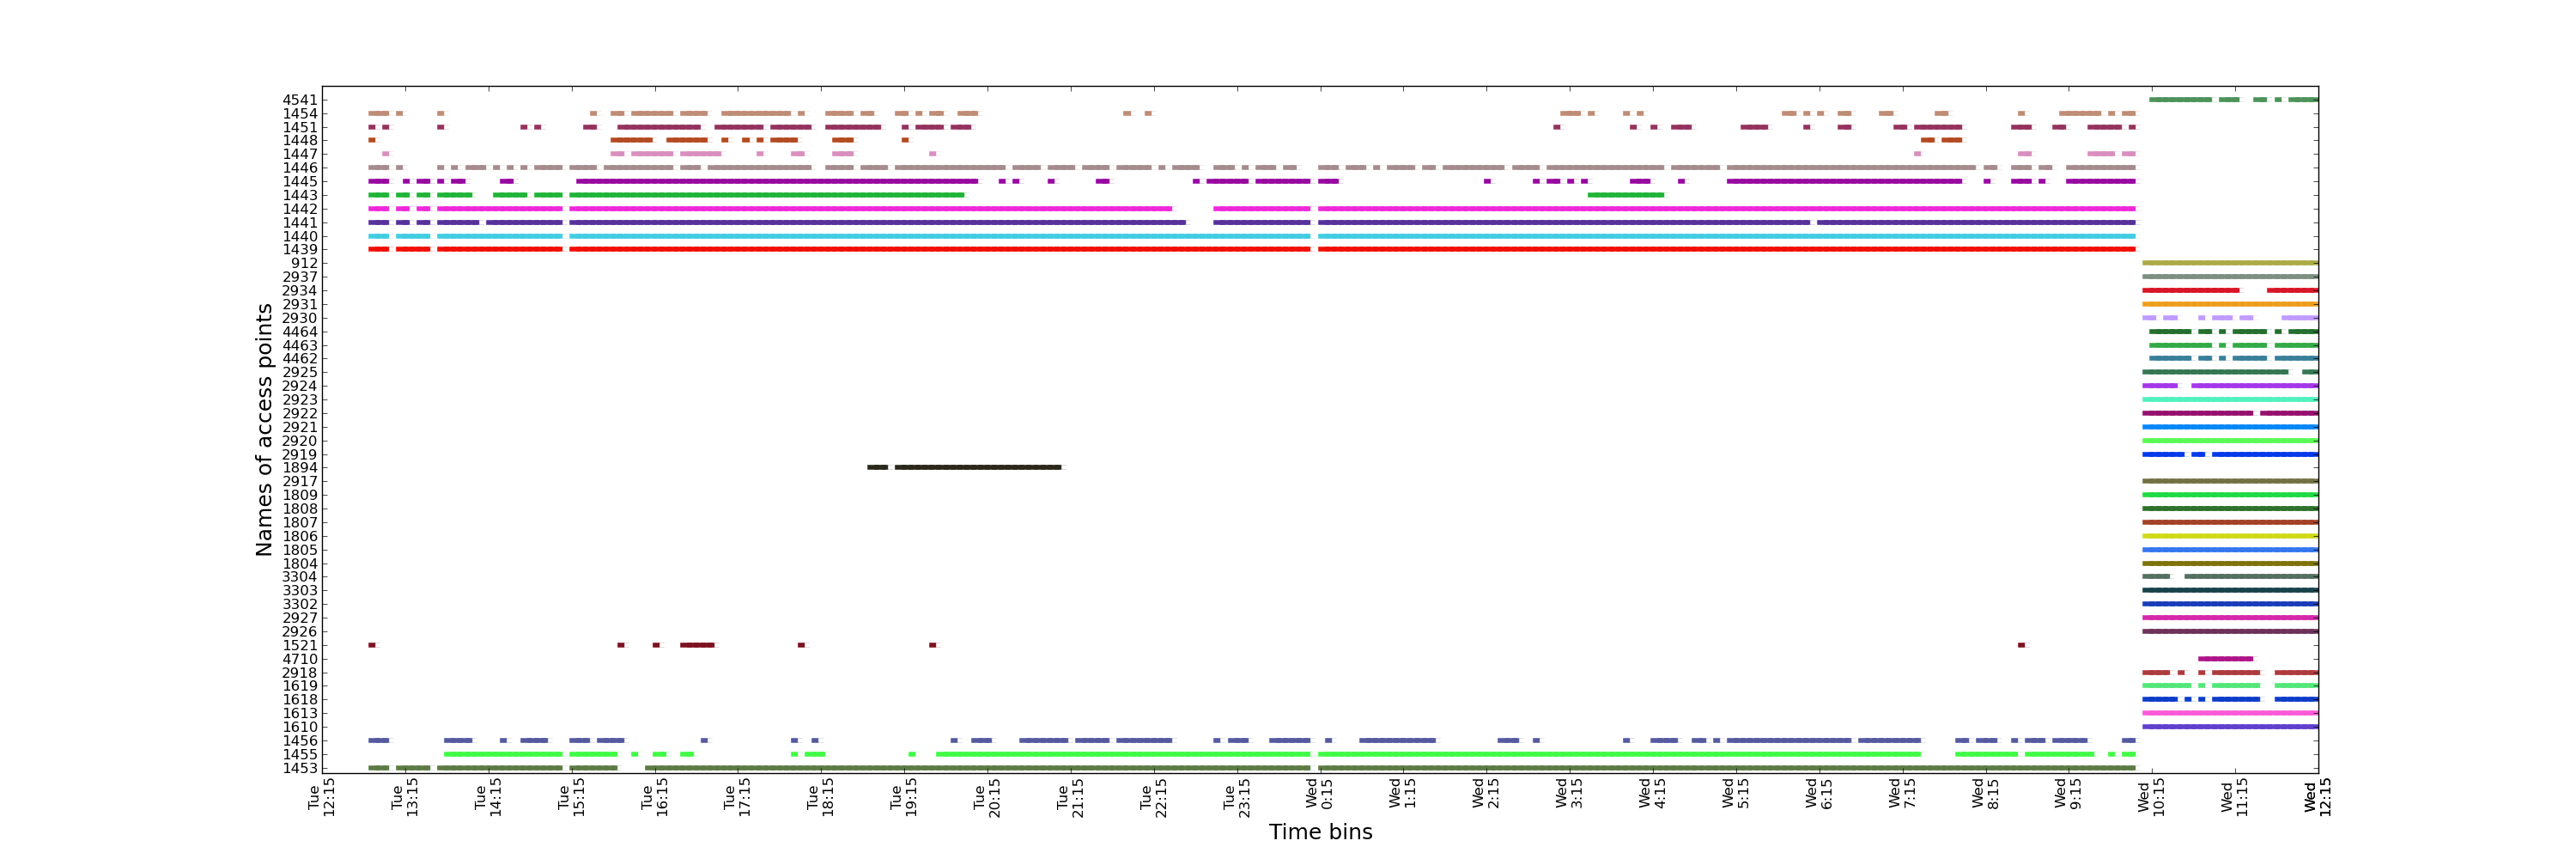
\includegraphics[width=1\textwidth]{figures/networks/user_6_sorted_1days_no_rssi_plot.png}
\caption{The most common 50 APs for userX during one day scan records}
\label{user_6_pres_1d}
\end{figure}

When running the algorithm that extract the locations based on the constructed
network, we obtain $21$ connected components which have the potential of being
locations. The image for the connected components can be seen in
Fig.~\ref{user_6_networks_1d} 

\begin{figure}[!h]
\centering
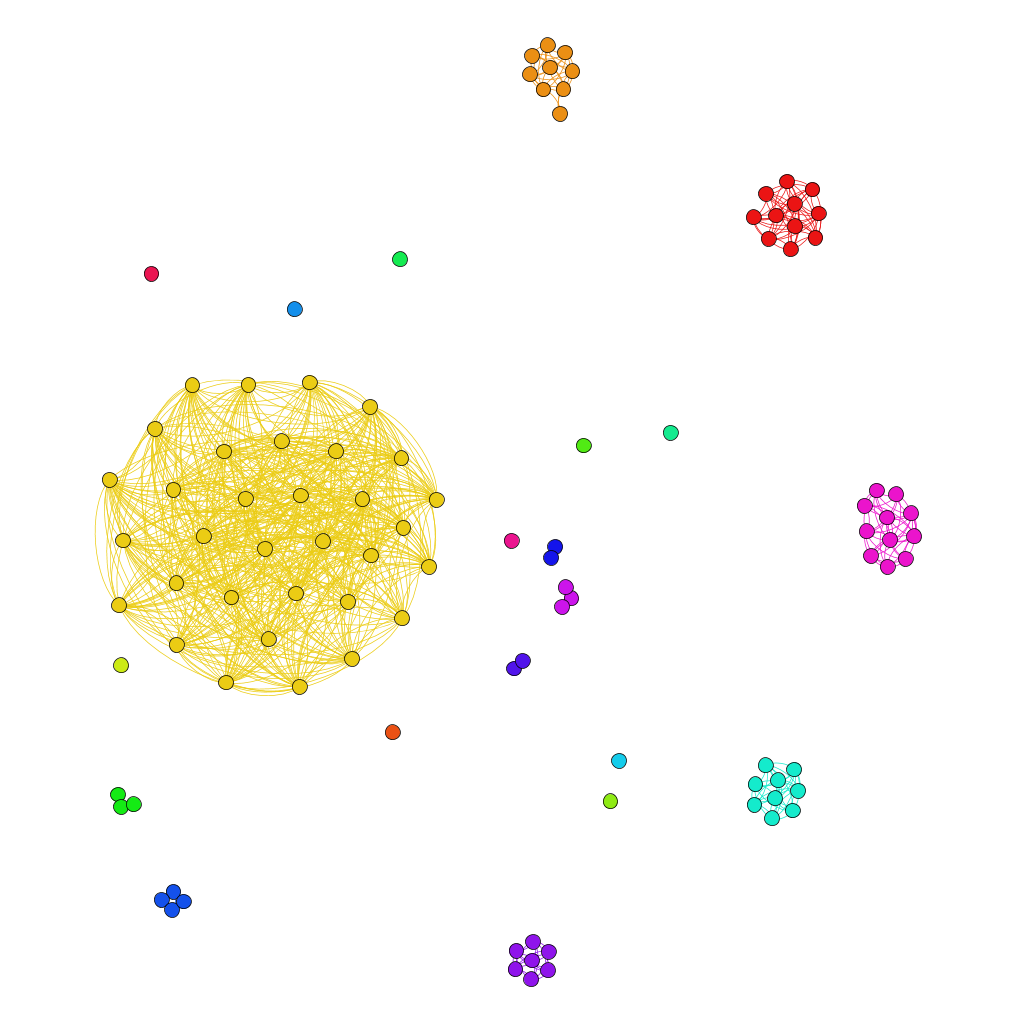
\includegraphics[width=1\textwidth]{figures/networks/user_6_day0_networks.png}
\caption{Locations identified with networks for userX during one day}
\label{user_6_networks_1d}
\end{figure}

We have tried to adjust the threshold for eliminating weak links yet the results
are in most cases unsatisfactory. Upon closer analysis we have observed that
this can be cause by the fact that, sometimes, there are a high number of APs
that even though they are in reality tied to a given location, their signal
fluctuates often and as such, the algorithm identifies them as part of a
different location and as such we have locations consisting in only a very small
number of APs that in reality could have been integrated in other locations.
This observation is sustained by the size distribution of the generated networks
(example for such a size distribution determined for the network in
Fig.~\ref{user_6_networks_1d} can be seen in
Fig.~\ref{user_6_size_distribution_1d}). Another thing we have observed is that
there are adjacent locations which can have interfering APs signals. This means
that our original supposition that, at all times, the APs that are visible from
a location will stop being visible in any other location does not always hold.

\begin{figure}[!h]
\centering
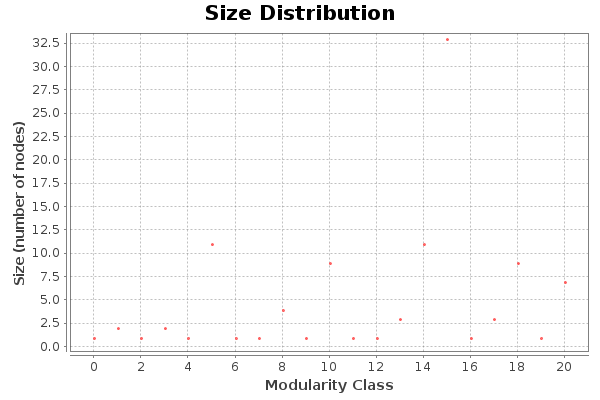
\includegraphics[width=0.7\textwidth]{figures/networks/communities-size-distribution.png}
\caption{Size distribution of locations based on the number of APs associated to
them }
\label{user_6_size_distribution_1d}
\end{figure}

For generating the networks and the size distributions, we have been using
Gephi~\cite{Gephi}. For visualizing the visualization in
Fig.~\ref{user_6_networks_1d} we have used the Force Atlas $2$ layer which has
been configured in order to avoid overlapping of components.

\subsection{K-means algorithm}
\subsection{Hidden Markov Models}
\section{Location matching}

\begin{enumerate}
  \item identifying locations
	\begin{itemize}
		\item Hidden Markov Models (5) 
		\item K-means(2)
	\end{itemize}
  \item matching locations locations (0.5)
	\begin{itemize}
		\item Percentage similarity (0.5)
		\item Keeping track of previous locations (0.5)
		\item Creating fingerprints (1.5)
	\end{itemize}
  \item  
\end{enumerate}